\chapter{Accepttest of Frequency response}\label{app:journal_Frequency_Response}
The purpose of this test is verify requirement \textbf{XX} concerning the linearity of the frequence responce of the system.

\section{Setup}
The setup of this test are depicted in \autoref{fig:AcceptFreqResponse}, where the equipment is catalogued in tab:UsedEquipmentFreqResponse, and described as follows:

\begin{itemize}
\item Frequency response will be measured by a Harmonie analyzer.
\item A noise generator will generate the following for the test. 
\begin{itemize}
\item Sampling frequency: 48000 Hz.
\item Generator amplitude: \textbf{X} V.
\item Pink noise.
\end{itemize}
\item The software of the system used for the bypass test is found at CD. \path{CD://Software/SystemFinal}

\end{itemize}


\subsection*{Test Setup}
\begin{figure}[H]
\centering
\includegraphics[width=0.9\textwidth]{FreqReponseSetup.png}
\label{fig:AcceptFreqResponse}
\caption{Test setup.}
\end{figure}

\subsection*{Equipment used and AAU-no.}

\begin{table}[H]
\centering
\ra{1.3}
\begin{tabular}{S[table-format=1]ccc} \toprule
    {Item} & {Description} & {AAU-no} \\ \bottomrule 
    1      &  Harmonie  & 60923  \\ 
    2      &  Harmonie PC  & 56524  \\ 
    3      &  Sine/Noise generator type 1049  & 08233  \\  \bottomrule 
\end{tabular}
\caption{Table over equipment used in the test}
\label{tab:UsedEquipmentFreqResponse}
\end{table}
\vspace{-5mm}


\section{Procedure}
The procedure for this experiment is described as follows:
\vspace{-5mm}
\begin{enumerate}
\item Setup the noise generator with the mentioned settings.
\item Setup the Harmonie and the Harmonie PC
\item Start recording on the PC
\item When finished save the results of the test.
\end{enumerate}

\section{Data Extraction}
The raw dat for the Bypass can be found at the CD \todo[inline]{CD}
The raw dat for the Full system can be found at the CD \todo[inline]{CD}
There are 30 bands from 20 Hz to 20 kHz, see \autoref{tb:freqBands}, where a magnitude is given in dB for each band. 10 different measurements have been taken for both bypass and the full system. The mean and standard deviation (std) have been found for each band as has been plotted. The two bands 25 Hz and 20000 Hz has been removed from the plots because of large deviation and therefore not deemed usefull.

\begin{table}[H]
\centering
\begin{tabular}{|c|c|c|c|c|c|c|c|c|c|}
\hline
\multicolumn{10}{|c|}{Bands [Hz]}                                       \\ \hline
25   & 31.5 & 40   & 50   & 63   & 80   & 100   & 125   & 160   & 200   \\ \hline
250  & 315  & 400  & 500  & 630  & 800  & 1000  & 1250  & 1600  & 2000  \\ \hline
2500 & 3150 & 4000 & 5000 & 6300 & 8000 & 10000 & 12500 & 16000 & 20000 \\ \hline
\end{tabular}
\caption{Frequency bands.}
\label{tb:freqBands}
\end{table}

\section{Analysis}

\begin{figure}[H]
	\centering
	\tikzsetnextfilename{FreqRespBypass}
	% This file was created by matlab2tikz.
%
%The latest updates can be retrieved from
%  http://www.mathworks.com/matlabcentral/fileexchange/22022-matlab2tikz-matlab2tikz
%where you can also make suggestions and rate matlab2tikz.
%
\definecolor{mycolor1}{rgb}{0.00000,0.44700,0.74100}%
%
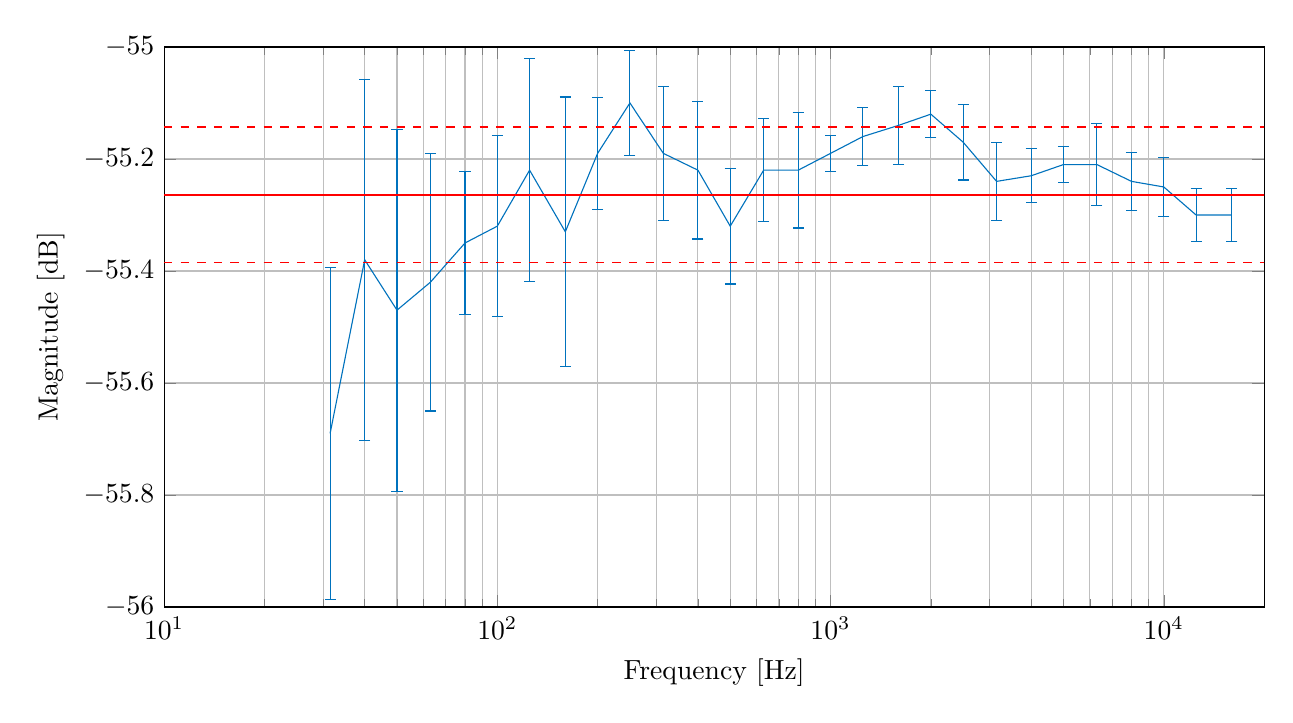
\begin{tikzpicture}

\begin{axis}[%
width=5.5in,
height=2.8in,
at={(0.758in,0.481in)},
scale only axis,
xmode=log,
xmin=10,
xmax=20000,
xminorticks=true,
xlabel={Frequency [Hz]},
xmajorgrids,
xminorgrids,
ymin=-56,
ymax=-55,
ylabel={Magnitude [dB]},
ymajorgrids,
axis background/.style={fill=white}
]
\addplot [color=mycolor1,solid,forget plot]
 plot [error bars/.cd, y dir = both, y explicit]
 table[row sep=crcr, y error plus index=2, y error minus index=3]{%
31.5	-55.69	0.296085573216034	0.296085573216034\\
40	-55.38	0.322490309931941	0.322490309931941\\
50	-55.47	0.323350515007408	0.323350515007408\\
63	-55.42	0.229975844142138	0.229975844142138\\
80	-55.35	0.126929551764397	0.126929551764397\\
100	-55.32	0.161932770686548	0.161932770686548\\
125	-55.22	0.198885785202351	0.198885785202351\\
160	-55.33	0.24060109910158	0.24060109910158\\
200	-55.19	0.0994428926011741	0.0994428926011741\\
250	-55.1	0.0942809041582077	0.0942809041582077\\
315	-55.19	0.119721899973785	0.119721899973785\\
400	-55.22	0.12292725943057	0.12292725943057\\
500	-55.32	0.103279555898863	0.103279555898863\\
630	-55.22	0.0918936583472665	0.0918936583472665\\
800	-55.22	0.103279555898863	0.103279555898863\\
1000	-55.19	0.0316227766016842	0.0316227766016842\\
1250	-55.16	0.051639777949433	0.051639777949433\\
1600	-55.14	0.0699205898780111	0.0699205898780111\\
2000	-55.12	0.042163702135579	0.042163702135579\\
2500	-55.17	0.0674948557710547	0.0674948557710547\\
3150	-55.24	0.0699205898780077	0.0699205898780077\\
4000	-55.23	0.048304589153962	0.048304589153962\\
5000	-55.21	0.031622776601682	0.031622776601682\\
6300	-55.21	0.0737864787372603	0.0737864787372603\\
8000	-55.24	0.0516397779494293	0.0516397779494293\\
10000	-55.25	0.05270462766947	0.05270462766947\\
12500	-55.3	0.0471404520791022	0.0471404520791022\\
16000	-55.3	0.0471404520791022	0.0471404520791022\\
};
\addplot [color=red,solid,forget plot]
  table[row sep=crcr]{%
10	-55.2642857142857\\
100000	-55.2642857142857\\
};
\addplot [color=red,dashed,forget plot]
  table[row sep=crcr]{%
10	-55.1429527298104\\
100000	-55.1429527298104\\
};
\addplot [color=red,dashed,forget plot]
  table[row sep=crcr]{%
10	-55.3856186987611\\
100000	-55.3856186987611\\
};
\end{axis}
\end{tikzpicture}%
	\caption{Frequency reposnse of bypassed signal with std´s. Mean=-55.264 dB (red line). Std=$\pm$0.121 dB (dashed red line).}
	\label{fig:FreqRespBypass}
\end{figure}

\begin{figure}[H]
	\centering
	\tikzsetnextfilename{FreqRespSystem}
	% This file was created by matlab2tikz.
%
%The latest updates can be retrieved from
%  http://www.mathworks.com/matlabcentral/fileexchange/22022-matlab2tikz-matlab2tikz
%where you can also make suggestions and rate matlab2tikz.
%
\definecolor{mycolor1}{rgb}{0.00000,0.44700,0.74100}%
%
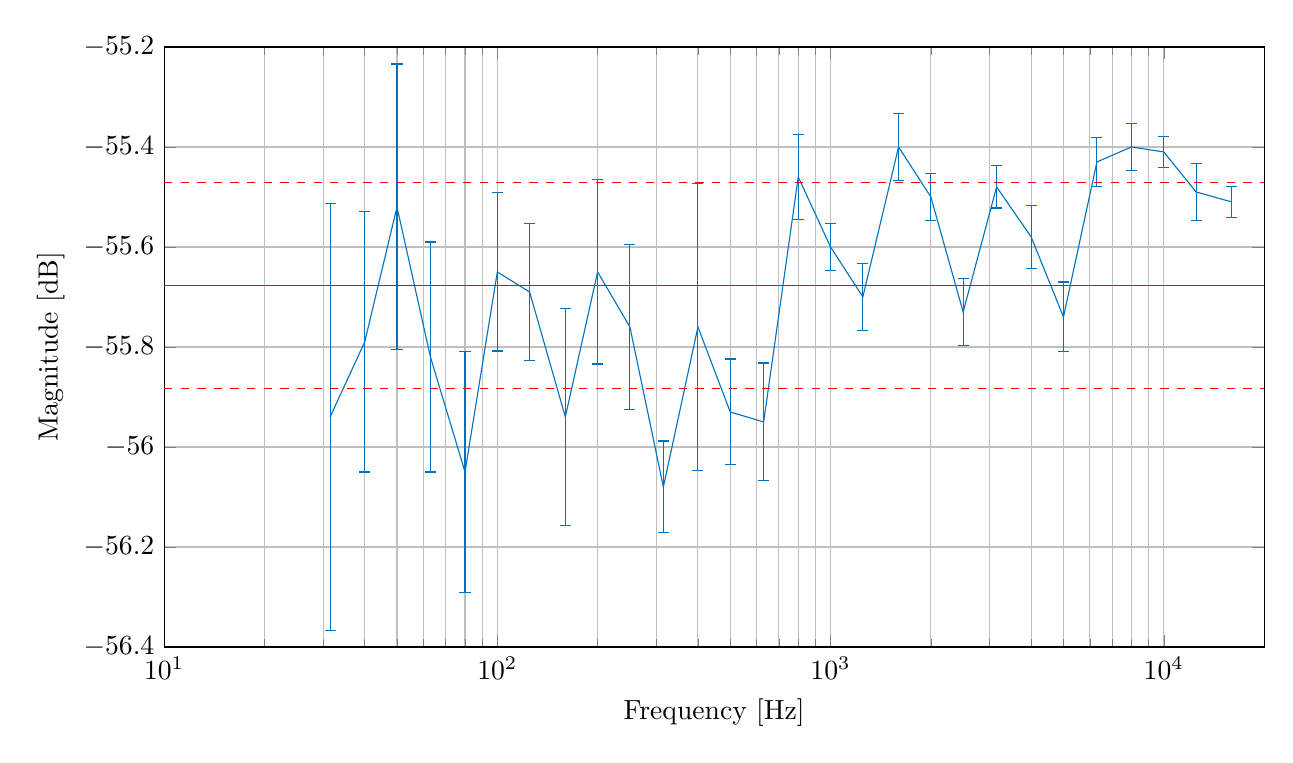
\begin{tikzpicture}

\begin{axis}[%
width=5.5in,
height=3.0in,
at={(0.758in,0.481in)},
scale only axis,
xmode=log,
xmin=10,
xmax=20000,
xminorticks=true,
xlabel={Frequency [Hz]},
xmajorgrids,
xminorgrids,
ymin=-56.4,
ymax=-55.2,
ylabel={Magnitude [dB]},
ymajorgrids,
axis background/.style={fill=white}
]
\addplot [color=mycolor1,solid,forget plot]
 plot [error bars/.cd, y dir = both, y explicit]
 table[row sep=crcr, y error plus index=2, y error minus index=3]{%
31.5	-55.94	0.427395211328656	0.427395211328656\\
40	-55.79	0.260128173535023	0.260128173535023\\
50	-55.52	0.285968141193696	0.285968141193696\\
63	-55.82	0.229975844142138	0.229975844142138\\
80	-56.05	0.241522945769825	0.241522945769825\\
100	-55.65	0.158113883008418	0.158113883008418\\
125	-55.69	0.137032031940629	0.137032031940629\\
160	-55.94	0.21705094128133	0.21705094128133\\
200	-55.65	0.184089350286454	0.184089350286454\\
250	-55.76	0.164654520469712	0.164654520469712\\
315	-56.08	0.0918936583472695	0.0918936583472695\\
400	-55.76	0.287518115371304	0.287518115371304\\
500	-55.93	0.10593499054714	0.10593499054714\\
630	-55.95	0.11785113019776	0.11785113019776\\
800	-55.46	0.084327404271158	0.084327404271158\\
1000	-55.6	0.0471404520791038	0.0471404520791038\\
1250	-55.7	0.0666666666666653	0.0666666666666653\\
1600	-55.4	0.0666666666666676	0.0666666666666676\\
2000	-55.5	0.0471404520791038	0.0471404520791038\\
2500	-55.73	0.0674948557710535	0.0674948557710535\\
3150	-55.48	0.042163702135579	0.042163702135579\\
4000	-55.58	0.0632455532033685	0.0632455532033685\\
5000	-55.74	0.0699205898780079	0.0699205898780079\\
6300	-55.43	0.0483045891539655	0.0483045891539655\\
8000	-55.4	0.0471404520791038	0.0471404520791038\\
10000	-55.41	0.0316227766016842	0.0316227766016842\\
12500	-55.49	0.0567646212197555	0.0567646212197555\\
16000	-55.51	0.0316227766016842	0.0316227766016842\\
};
\addplot [color=red,solid,forget plot]
  table[row sep=crcr]{%
10	-55.6771428571429\\
100000	-55.6771428571429\\
};
\addplot [color=red,dashed,forget plot]
  table[row sep=crcr]{%
10	-55.4716469412989\\
100000	-55.4716469412989\\
};
\addplot [color=red,dashed,forget plot]
  table[row sep=crcr]{%
10	-55.8826387729869\\
100000	-55.8826387729869\\
};
\end{axis}
\end{tikzpicture}%
	\caption{Frequency reposnse of full system signal with std´s. Mean=-55.677 dB (red line). Std=$\pm$0.205 dB (dashed red line).}
	\label{fig:FreqRespSystem}
\end{figure}

\begin{figure}[H]
	\centering
	\tikzsetnextfilename{FreqRespComp}
	% This file was created by matlab2tikz.
%
%The latest updates can be retrieved from
%  http://www.mathworks.com/matlabcentral/fileexchange/22022-matlab2tikz-matlab2tikz
%where you can also make suggestions and rate matlab2tikz.
%
\definecolor{mycolor1}{rgb}{0.00000,0.44700,0.74100}%
\definecolor{mycolor2}{rgb}{0.85000,0.32500,0.09800}%
%
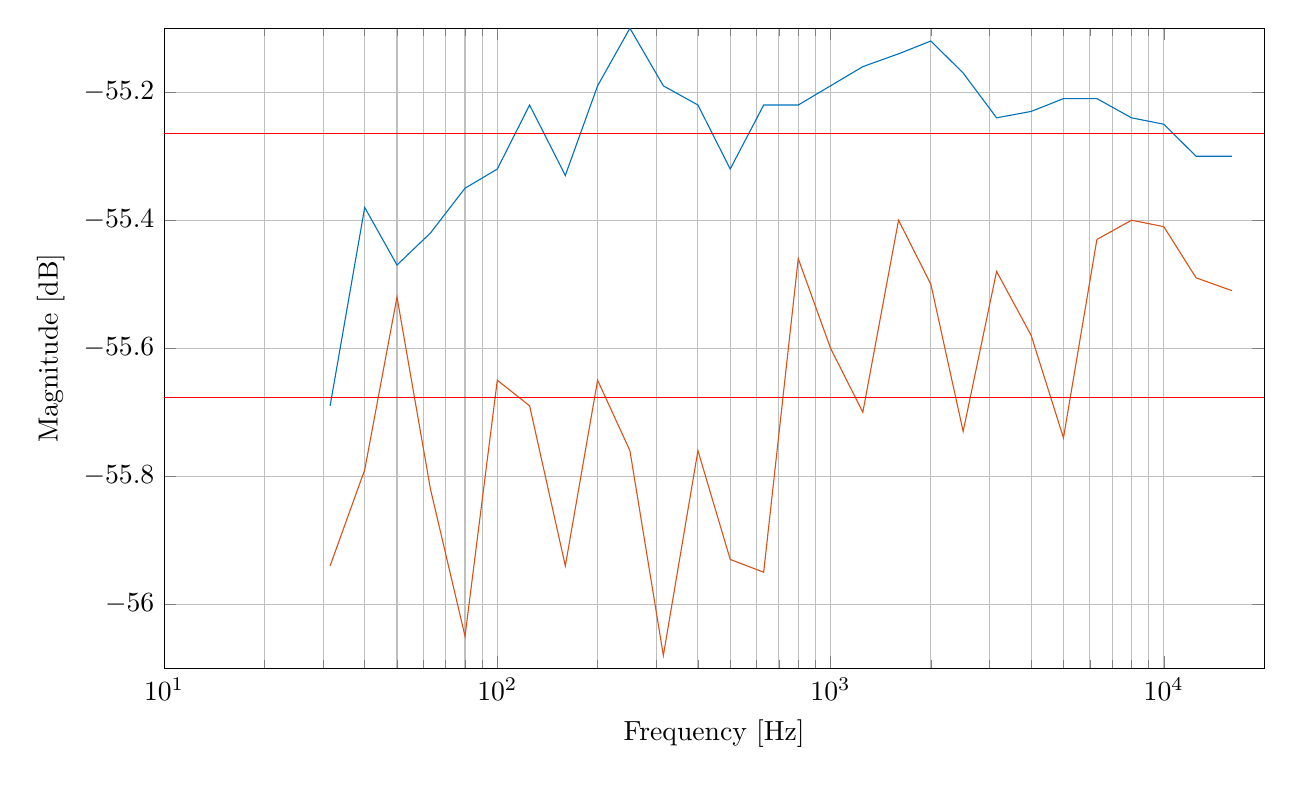
\begin{tikzpicture}

\begin{axis}[%
width=5.5in,
height=3.2in,
at={(0.758in,0.481in)},
scale only axis,
xmode=log,
xmin=10,
xmax=20000,
xminorticks=true,
xlabel={Frequency [Hz]},
xmajorgrids,
xminorgrids,
ymin=-56.1,
ymax=-55.1,
ylabel={Magnitude [dB]},
ymajorgrids,
axis background/.style={fill=white}
]
\addplot [color=mycolor1,solid,forget plot]
  table[row sep=crcr]{%
31.5	-55.69\\
40	-55.38\\
50	-55.47\\
63	-55.42\\
80	-55.35\\
100	-55.32\\
125	-55.22\\
160	-55.33\\
200	-55.19\\
250	-55.1\\
315	-55.19\\
400	-55.22\\
500	-55.32\\
630	-55.22\\
800	-55.22\\
1000	-55.19\\
1250	-55.16\\
1600	-55.14\\
2000	-55.12\\
2500	-55.17\\
3150	-55.24\\
4000	-55.23\\
5000	-55.21\\
6300	-55.21\\
8000	-55.24\\
10000	-55.25\\
12500	-55.3\\
16000	-55.3\\
};
\addplot [color=mycolor2,solid,forget plot]
  table[row sep=crcr]{%
31.5	-55.94\\
40	-55.79\\
50	-55.52\\
63	-55.82\\
80	-56.05\\
100	-55.65\\
125	-55.69\\
160	-55.94\\
200	-55.65\\
250	-55.76\\
315	-56.08\\
400	-55.76\\
500	-55.93\\
630	-55.95\\
800	-55.46\\
1000	-55.6\\
1250	-55.7\\
1600	-55.4\\
2000	-55.5\\
2500	-55.73\\
3150	-55.48\\
4000	-55.58\\
5000	-55.74\\
6300	-55.43\\
8000	-55.4\\
10000	-55.41\\
12500	-55.49\\
16000	-55.51\\
};
\addplot [color=red,solid,forget plot]
  table[row sep=crcr]{%
10	-55.6771428571429\\
100000	-55.6771428571429\\
};
\addplot [color=red,solid,forget plot]
  table[row sep=crcr]{%
10	-55.2642857142857\\
100000	-55.2642857142857\\
};
\end{axis}
\end{tikzpicture}%
	\caption{Frequency reposnse of bypassed and full system signal. Bypass (blue), Full system (Orange), mean difference = 0.4130 dB}
	\label{fig:FreqRespComp}
\end{figure}

\section{Error sources}


\section{Conclusion}
From the test of bypass and fulle system it can be concluded that 